% ============================================================
% Mechatronics Submission — RoboParts: Three-State Honesty
% Template: elsarticle-num (Elsevier numbered references)
% Compile: pdflatex main.tex && bibtex main && pdflatex x2
% ============================================================
\documentclass[review]{elsarticle}
\usepackage{lineno}        % line numbers for review
\usepackage{amsmath,amssymb,amsfonts}
\usepackage{graphicx}
\usepackage{booktabs}      % booktabs for tables
\usepackage{xcolor}
\usepackage{hyperref}
\usepackage{url}
\usepackage{array}
\usepackage{enumitem}

\journal{Mechatronics}

% ============================================================
% Title & Authors
% ============================================================
\begin{document}
\begin{frontmatter}

\title{Three-State Honesty in Robotic Hardware Compatibility:
       A Vendor-Neutral Determination Layer}

\author[inst1]{Lexing Li\fnref{fn1}}
\cortext[cor1]{Corresponding author.}
\ead{TODO_email}

\affil[inst1]{%
  % TODO: 请补充单位全称（若属无依托研究可写
  % "Independent Researcher, China"）
  TODO_affiliation
}

\fntext[fn1]{ORCID: \url{https://orcid.org/0009-0004-2152-7669}}

\begin{abstract}
Compatibility determination between robotic hardware components is the
foundational yet most fragile step in the supply chain of embodied AI.
Existing engineering practice addresses "can this part be mounted on
that?" through three unsatisfactory routes: free-form documentation,
bill-of-materials and trial-and-error, or vendor-private compatibility
matrices. All three are binary — either \emph{yes} or \emph{no} —
although real engineering is filled with combinations that must be
labelled \emph{unknown}. The forced binary answer causes two symmetric
errors: false-positive compatibility (mechanical damage, personal
injury) and false-negative compatibility (wasted integration time).

We present \textbf{RoboParts}, a vendor-neutral determination layer
that formalises compatibility as a three-valued function over a
three-axis type system:
$\mathsf{compose}(a,b) \in \{\mathsf{composed}, \mathsf{type\_error}, \mathsf{unknown}\}$,
with the design choice that \emph{unknown} takes priority over
\emph{composed} — ignorance is a first-class citizen, not a null value.
The mechanical axis inherits reflexivity (same standard implies
compatibility) only for \emph{geometric-spec} types; it is deliberately
withdrawn for \emph{directional-role} types (e.g.\ \texttt{OUTPUT\_SPIKE},
where two matching instances are not complementary). The electrical and
signal axes are evaluated independently.

Across $802$ real-world robotic entities yielding $351{,}649$ full
pair evaluations, we observe $\mathsf{composed}=0$,
$\mathsf{type\_error}=4$, $\mathsf{unknown}=351{,}645$ — a coverage
map, not a benchmark failure. We introduce \emph{gap-distance} and
\emph{d1-bottleneck} measures that turn the $unknown$ mass into an
actionable data-flywheel priority queue: all $112$ pairs at
$d=1$ are bottlenecked on the electrical axis alone. A three-class gap
causation taxonomy (unpublished/proprietary/ambiguous) together with
a manufacturer concentration analysis shows that top-10 out of 242
vendors account for only $28.5\%$ of the coverage gap, ruling out
"crawl a few datasheets" as a viable closure strategy and pointing
to user-submission and open-source-BOM reverse-feeding as the
only scalable paths.
\end{abstract}

\begin{keyword}
Robotic hardware compatibility \sep vendor-neutral knowledge layer \sep
three-valued reasoning \sep engineering ontology \sep
data-flywheel prioritisation \sep knowledge-graph
\end{keyword}

\end{frontmatter}

% ============================================================
% Highlights — 5 bullets, each ≤ 85 characters
% TODO: 提交时另附 highlights.txt
% ============================================================
% 1. Compatibility is three-valued, not binary.
% 2. Unknown outranks Composed — ignorance is a first-class citizen.
% 3. Reflexivity holds for geometric spec types only, not directional roles.
% 4. 5.69% mechanical declaration rate is a coverage map, not a failure.
% 5. gap-distance and d1-bottleneck turn unknowns into a data-flywheel queue.

% ============================================================
% Declaration of generative AI use
% ============================================================
\section*{Declaration of generative AI and AI-assisted technologies
in manuscript preparation}
During the preparation of this manuscript, the authors used
\textbf{ChatGPT-4o} and \textbf{DeepSeek} for language editing and
figure captions only. All scientific claims, formalisations,
experiments, and dataset statistics were produced, verified, and
reproducible without AI assistance. All authors have reviewed and
approved the final manuscript and take full responsibility for
its content.

\section*{Declaration of competing interest}
The authors declare that they have no known competing financial
interests or personal relationships that could have appeared to
influence the work reported in this paper.

\section*{Data availability}
All data, code and intermediate artefacts used to produce the results
reported in this paper are released under MIT (code) and CC BY 4.0
(data) at \url{https://github.com/lm203688/roboparts}. The dataset
snapshot referenced by this manuscript is commit
\texttt{50a2e012} and the API outputs (\texttt{entities.json},
\texttt{gap_classification.json}, \texttt{compose_semantics.json},
\texttt{morphology_graph.json}) are frozen at that revision.

% ============================================================
% 1. Introduction
% ============================================================
\section{Introduction}

The next bottleneck in embodied AI is not how smart a robot is, but
what it can be \emph{attached} to. A representative open-source arm
project (\textsc{Seeed reBot-DevArm}~\cite{R14}) publishes STEP files,
BOMs, a Python SDK, ROS\,2 integration, LeRobot tutorials and Isaac-Sim
simulations — four layers complete — but does not answer the question
``can this end-effector mount on this wrist, and can this sensor talk
to this mainboard?'' Compatibility determination has, for years,
lived as prose documentation, private vendor matrices, or manual
trial-and-error, with no neutral, machine-readable, decidable public
layer.

The central claim of this paper is that the correct semantics of
compatibility are not two-valued but \emph{three-valued}. ``I know
it works'' and ``I know it does not work'' are both evidence states;
``I do not know'' is a third evidence state, and it is the one that
tells you exactly which declaration to fill in and how many unknowns
that fills close. Ignoring this third state produces two symmetric,
costly errors:

\begin{itemize}[nosep,leftmargin=*]
\item \textbf{False-positive compatibility} — treating ``not found''
as ``yes'': mechanical damage, electrical failure, personal injury.
\item \textbf{False-negative compatibility} — treating ``not found''
as ``no'': hours of trial-and-error on combinations that in fact
work.
\end{itemize}

Our design principle is \emph{three-state honesty}: compatibility
is a function
\begin{equation}
  \mathsf{compose}(a, b) \;\in\;
  \{\mathsf{composed},\ \mathsf{type\_error},\ \mathsf{unknown}\}
  \label{eq:trivalue}
\end{equation}
where $\mathsf{unknown}$ \emph{outranks} $\mathsf{composed}$ — if
any of the three axes lacks evidence, the composite verdict is
$\mathsf{unknown}$. This is the sharp dividing line from every binary
compatibility matrix.

Vendor-neutrality is the second, non-negotiable design constraint:
RoboParts does not manufacture, resell, or take commission on any
part, and has no commercial tie to any listed vendor. A compatibility
layer with a monetary interest in one of the two queried parts has
an incentive to be wrong.

\paragraph{Contributions.}
\begin{enumerate}[nosep]
\item A three-valued compatibility function over a three-axis type
system (mechanical / electrical / signal), with an explicit
\emph{reflexivity boundary} — same-type means compatible only for
geometric-specification types (e.g.\ ISO 9409-1 flange sizes), and is
deliberately withdrawn for directional-role types
(\texttt{OUTPUT\_SPIKE}, \texttt{INPUT\_SENSORY}), where two matching
instances are complementary only if their roles differ.

\item A coverage map of $802$ robotic entities and $351{,}649$ full
pair evaluations yielding $5.69\%$ mechanical declaration rate —
deliberately reported as an \emph{honesty baseline} rather than
a benchmark.

\item Two new measures, \emph{gap-distance} ($d$ = number of axes
that returned $\mathsf{unknown}$ for a pair) and \emph{d1-bottleneck}
(axis responsible when $d=1$), which turn the $\mathsf{unknown}$ mass
into an actionable data-flywheel priority queue. On our corpus,
$100\%$ of the $112$ $d=1$ pairs are bottlenecked on the electrical
axis, giving an unambiguous next step.

\item A three-class gap-causation taxonomy
(unpublished-suspect $350$ / proprietary-suspect $5$ / ambiguous $59$)
together with a manufacturer concentration analysis ($242$ vendors,
top-$10$ accounting for $28.5\%$ of the gap). This is
\emph{negative evidence}: the coverage gap cannot be closed by
crawling a small number of vendor datasheets. The only scalable paths
are user-submission, OSS-BOM reverse-feeding, and community pull-requests.
\end{enumerate}

\paragraph{Paper outline.}
Section~2 surveys related work in assembly-graph learning, engineering
ontologies, and uncertainty-aware robot learning. Section~3 gives the
formal definitions. Section~4 describes the corpus. Section~5 reports
experiments. Section~6 discusses limitations and the reflexivity
boundary in depth. Section~7 concludes.

% ============================================================
% 2. Related Work
% ============================================================
\section{Related Work}

\subsection{Standards and the missing decision layer}

The three-axis backbone of RoboParts is deliberately thin on standards.
\textsc{ISO 9409-1}~\cite{iso9409} defines the canonical letter codes
(\texttt{A55} through \texttt{H350}) for the flange sizes used in
industrial manipulation devices. \textsc{ISO 3025}~\cite{iso3025}
fixes dowel-hole positions for those flanges. \textsc{ISO 9653}~\cite{iso9653}
covers safety-critical cylinder interfaces. What these standards
\emph{do not} define is the third axis — a signal-level type system
that lets two independently-produced devices be checked for whether
their roles are complementary. That gap is the reason that the
existence of a common flange is not sufficient to certify a mating
pair: two devices can share an \texttt{A55} flange and still be
electrical incompatible, or signal-direction incompatible.

We are not alone in wanting a machine-readable decision layer. The
\textsc{STEP-NC} framework for additive manufacturing~\cite{R12}
unifies geometry, material and process parameters into a single
digital spine, but at the \emph{manufacturing-process} scale, not the
selection-scale. \textsc{ANSI}'s survey of additive standards
\cite{R13} emphasises that standardisation has three components —
terminology alignment, data exchange, and test methods — and
that all three must be present for the layer to be useful. RoboParts
addresses terminology (three-axis type system), data exchange
(machine-readable \texttt{entities.json}), and test methods
(arithmetic crosscheck invariants) — but does not yet address the
\emph{calibration} step, which is the subject of Section~6.4.

\subsection{Assembly graphs and interface geometry}

The closest geometric neighbours to our work are assembly-graph
learners. \textsc{Linkify}~\cite{R1} re-computes high-fidelity
contact points for Fusion-360-Gallery assemblies and trains a GATv2
on top of point-cloud encoded interfaces, achieving strong masked-part
prediction. Harlacher \& Friedrich~\cite{R2} learn geometric relation
labels from point clouds and then convert them into symbolic assembly
graphs, achieving $85.8\%$ success on \textsc{ASAP} with human-in-the-loop
correction. Semantic enrichment via LLM-annotated scene graphs over
CAD data~\cite{R3} takes the CAD-uncertainty direction: when the
annotator is uncertain, the annotator's uncertainty is preserved in
the graph. All three operate at the \emph{geometric} layer of
interfaces. RoboParts operates at the \emph{semantic} layer — types,
declarations, and unknowns — and is complementary to (not
competitive with) these methods. A geometry learner that trusts its
own point clouds can only ever tell you what it saw; RoboParts is
what tells you what it \emph{has not yet seen}.

A systematic study of machine learning on assembly guidance ontologies
\cite{R8} shows that AR-assisted assembly guidance benefits from
ontology-driven retrieval, but again operates on a fixed set of known
parts. \textsc{ExtruOnt}~\cite{R5} provides a formal ontology for
extrusion machines covering components, spatial connections, features
and sensors, and is a direct model of the ontology-driven approach we
adopt at the entity level. Ontology-based KGs for systems engineering
\cite{R6} and for robot manipulation with geometric constraints~\cite{R7}
both operate at the \emph{single-machine} scale. The unified graph
framework for industrial-robot automatic design~\cite{R4} pushes
toward design-time KGs that recommend parts — the dual of what we do
at query time. A systematic review of ontology-plus-ML research
\cite{R9} identifies this same cross-connection between ontology
definitions and downstream machine-learning pipelines, which is the
motivating background for RoboParts.

\subsection{Uncertainty-aware robot learning}

On the decision side, \textsc{ReconVLA}~\cite{R10} uses conformal
prediction intervals to give vision-language-action policies explicit
coverage guarantees, letting the planner refuse when the interval
is too wide. The VLA uncertainty survey~\cite{R11} makes the same
argument at a higher level: a policy that returns \emph{I don't know}
is strictly better than one that guesses when guessing is more
costly than deferring. RoboParts brings the same three-valued
philosophy to the \emph{data} layer rather than the \emph{decision}
layer. The stack reads bottom-up as: \emph{data layer three-state
(compatibility)} $\rightarrow$ \emph{reasoning layer KG (assembly
planning)} $\rightarrow$ \emph{decision layer UQ (policy refusal)}.
Each layer's unknown feeds the previous one's priority queue.

\subsection{Open-source hardware and BOM semantics}

Two representative open-source arm/hand projects show the current
state of vendor-published hardware data. \textsc{Seeed reBot-DevArm}~\cite{R14}
ships STEP files, a BOM, Python SDK, ROS\,2 integration, LeRobot
tutorials, and Isaac-Sim simulations — but does not annotate any
interface on any part with a machine-readable type. \textsc{TetherIA
Aero Hand}~\cite{R15}, at $\$$314 per unit, is even more extreme:
a fully documented mechanical design with no interface metadata
whatsoever. RoboParts ingests both as OSS-BOM sources for reverse
feeding, but even after ingestion, $0\%$ of their parts have a full
three-axis declaration. This is the empirical reason we frame RoboParts
as a \emph{coverage map} rather than a benchmark.

\subsection{Hardware abstraction layers and modular robotics}

Recent work on hardware abstraction layers for modular robotic
synthesis~\cite{R16} and on modular robot assembly in general both
assume that the underlying parts are known and interoperable. Their
concern is composition-time behaviour, not selection-time
compatibility. RoboParts is upstream of these layers: it is what
tells them which parts to compose.

\subsection{Positioning}

To our knowledge, no prior work formalises a three-valued
compatibility function for robotic hardware at the vendor-neutral
scale. The closest is assembly-graph work, which by construction
operates on the specific assembly being assembled (i.e.\ known
components) rather than on the open world of independently
manufactured parts. RoboParts is orthogonal to, and complementary
with, every category above.

% ============================================================
% 3. Method
% ============================================================
\section{Method}

\subsection{The three-valued compatibility function}

Let $\mathcal{P}$ be the set of parts. We define the composite
function
\begin{equation}
  \mathsf{compose}(a, b) \;=\;
    \mathsf{agg}\!\bigl(\mathsf{ax}_1(a,b),\
    \mathsf{ax}_2(a,b),\ \mathsf{ax}_3(a,b)\bigr),
  \label{eq:compose}
\end{equation}
where the three axes $\mathsf{ax}_i : \mathcal{P}\times\mathcal{P}
\to \{\mathsf{composed}, \mathsf{type\_error}, \mathsf{unknown}\}$
are the \emph{mechanical}, \emph{electrical}, and \emph{signal}
axes. The aggregation rule is lexicographic with $\mathsf{unknown}$
above $\mathsf{composed}$:
\begin{equation}
  \mathsf{agg}(x_1, x_2, x_3) \;=\;
  \begin{cases}
    \mathsf{type\_error} & \text{if any } x_i = \mathsf{type\_error}\\
    \mathsf{unknown}     & \text{else if any } x_i = \mathsf{unknown}\\
    \mathsf{composed}    & \text{else.}
  \end{cases}
  \label{eq:agg}
\end{equation}
The rule ``$\mathsf{unknown}$ outranks $\mathsf{composed}$'' is the
single most important design choice: it means a system with no
evidence cannot accidentally certify compatibility.

\subsection{Axis definitions}

\paragraph{Mechanical axis.}
A part declares a mechanical interface as
$(\texttt{standard}, \texttt{class}, \texttt{role})$. \emph{Standards}
are drawn from ISO 9409-1 (robot flange sizes \texttt{A}--\texttt{H}),
ISO 3025 (dowel holes), ISO 9653 (cylinder), and a small set of
vendor-specific flange standards we do not attempt to normalise.
Two parts are \emph{mechanically} compatible iff they declare
mutually consistent values on the standard axis.

\paragraph{Reflexivity boundary.}
Same-standard implies same-interface implies compatibility is a
\emph{design assumption}, not a fact. It holds for
\emph{geometric-specification} types (any two \texttt{A}55 flanges
mating with a matching \texttt{A}55 interface are compatible by
construction). It does \emph{not} hold for \emph{directional-role}
types. Two parts both declaring \texttt{role = OUTPUT\_SPIKE} do not
form a mating pair — the mating partner of an \texttt{OUTPUT\_SPIKE}
is an \texttt{INPUT\_SENSORY} (or a \texttt{ACTUATOR\_DRIVE}), not
another output. The type table explicitly encodes:
\begin{equation}
  \mathsf{complement}\!\bigl(\texttt{OUTPUT\_SPIKE}\bigr) \;\subseteq\;
    \{\texttt{INPUT\_SENSORY},\ \texttt{ACTUATOR\_DRIVE}\}.
  \label{eq:complement}
\end{equation}
This boundary is what separates RoboParts from a naive "same label
equals match" scheme, and is the reason the same-\texttt{type} pair
in a morphology graph returns $\mathsf{type\_error}$ rather than
$\mathsf{composed}$.

\paragraph{Electrical axis.}
Connector pin count and pitch are the two hard constraints: pin-count
equality is required; pitch mismatch is a \emph{hard} incompatible
signal regardless of any other information. This axis is deliberately
thin — a full electrical ontology is a multi-year project.

\paragraph{Signal axis.}
Only for a small set of high-value categories do we declare roles
(\texttt{OUTPUT\_SPIKE}, \texttt{INPUT\_SENSORY}, \texttt{REWARD}).
\texttt{REWARD} is metadata and does not participate in positive
determination. The signal axis is thus sparse by design: its role is
to catch directionality errors that the mechanical axis cannot see.

\subsection{Gap-distance and d1-bottleneck}

For a pair $(a, b)$ with axis results $x_1, x_2, x_3 \in
\{\mathsf{composed}, \mathsf{type\_error}, \mathsf{unknown}\}$,
define
\begin{equation}
  d(a, b) \;=\; |\{\, i \;:\; x_i = \mathsf{unknown}\,\}|.
  \label{eq:gapd}
\end{equation}
A pair with $d=0$ has been fully determined by the current corpus;
a pair with $d=3$ has no evidence anywhere. The critical
operational quantity is $d=1$: a single declaration closes the pair.
We compute the axis responsible by attributing the $\mathsf{unknown}$
verdict to whichever axis returned it. When $d=1$ for a pair, the
axis responsible is uniquely defined; we call this the
\emph{d1-bottleneck}.

The pair corpus is thus converted into a priority queue: process
the $d=1$ population first, since each declaration closes one full
pair, and process $d=2$ second, etc. This gives an explicit,
monotonically-improvable data-flywheel, in contrast to the
undirected ``crawl more datasheets'' strategy.

\subsection{Pipeline implementation}

RoboParts is implemented as a set of independent operators on a
DAG (see Appendix~A of the source release for the operator
register). Each operator is a pure function with a single JSON
input and a single JSON output; failures are loud (exceptions
propagate). All 802 entities, all 439 mechanical-applicable pairs,
and all 351,649 composite evaluations are produced by the same
declarative pipeline in $<$ 4 seconds.

\subsection{Data model}

Each entity is a JSON object with three axes:

\begin{verbatim}
{
  "id": "a69b91f1",
  "category": "flange",
  "manufacturer": "Universal Robots",
  "part_name": "UR-e flange",
  "mechanical": { "standard": "A80", "class": "flange",
                  "role": "GEOMETRIC_SPEC",
                  "source_url": "https://...",
                  "evidence_tier": "vendor_datasheet" },
  "electrical": { "connector": "M12 5-pin",
                  "pin_count": 5, "pitch_mm": 3.8,
                  "source_url": null, "evidence_tier": "unknown" },
  "signal":     { "roles": ["OUTPUT_SPIKE"],
                  "source_url": null, "evidence_tier": "unknown" }
}
\end{verbatim}

Every axis carries an \texttt{evidence\_tier} field, one of
\texttt{vendor\_datasheet}, \texttt{iso\_table}, \texttt{user\_submission},
\texttt{oss\_bom}, \texttt{unknown}. The tier is a monotone ordering:
a lower-tier evidence never overrides a higher-tier evidence, but
may \emph{confirm} it. This is what makes the corpus upgrade-safe
— new evidence can be added without deleting existing higher-tier
evidence, and the crosscheck invariants of Section~5.4 continue to
hold.

\subsection{Reflexivity in the type table}

The type table is a small JSON file with four fields per role:
\texttt{role}, \texttt{kind} (either \texttt{GEOMETRIC\_SPEC} or
\texttt{DIRECTIONAL\_ROLE}), \texttt{complements} (a set of role names),
and \texttt{reflexive} (a boolean that is \texttt{true} iff the
role's \texttt{kind} is \texttt{GEOMETRIC\_SPEC}). The four $\mathsf{type\_error}$
verdicts in Table~\ref{tab:overall} all originate from a
self-pair of a role with \texttt{kind = DIRECTIONAL\_ROLE} — i.e.,
\texttt{OUTPUT\_SPIKE} mated with \texttt{OUTPUT\_SPIKE}. The
reflexivity boundary is thus not a special case in the algorithm;
it is a single field in the type table.

% ============================================================
% 4. Dataset
% ============================================================
\section{Dataset}

The corpus is drawn from public, licence-compatible sources: vendor
datasheets where the manufacturer publishes a machine-readable
interface declaration, ISO 9409-1 tables for flange size look-up,
and open-source bill-of-materials files from projects such as
\textsc{Seeed reBot-DevArm}~\cite{R14} and \textsc{TetherIA Aero
Hand}~\cite{R15}. The corpus is intentionally small
($802$ entities, $439$ applicable for the mechanical axis,
$25$ with a full declaration) because our goal is not scale but
\emph{honesty under scarcity}.

\begin{table}[ht]
\centering
\caption{Corpus composition and axis coverage.}
\label{tab:corpus}
\begin{tabular}{@{}llrr@{}}
\toprule
Axis       & Applicable & Declared & Rate \\
\midrule
Mechanical & 439        & 25       & 5.69\% \\
Electrical & 220        & 4        & 1.82\% \\
Signal     & 118        & 9        & 7.63\% \\
\bottomrule
\end{tabular}
\end{table}

Table~\ref{tab:corpus} reports the honest per-axis declaration rates.
The mechanical axis is the one we expect to be the most complete; the
fact that it stands at $5.69\%$ is the strongest single argument for
the three-state design — a binary compatibility layer built on this
corpus would be a coin flip.

\subsection{Gap causation taxonomy}

Of the 439 mechanically applicable entities, 414 lack a full
declaration. We classify each gap into one of three causes:

\begin{itemize}[nosep,leftmargin=*]
\item \textbf{unpublished-suspect} ($n=350$): the manufacturer
appears to have the data but has not made it publicly available in a
machine-readable form. \emph{Suspect} is used because we cannot
distinguish ``the vendor has never measured it'' from ``the vendor
has measured it but is not sharing it.''

\item \textbf{proprietary-suspect} ($n=5$): the part's mechanical
interface is genuinely non-standard (typically connector pinouts
specific to a single manufacturer). Reverse-engineering is technically
possible but legally risky.

\item \textbf{ambiguous} ($n=59$): the manufacturer publishes
something, but it cannot be uniquely mapped to our taxonomy without
further context (e.g.\ a datasheet that specifies ``standard flange,
see ISO 9409-1'' without saying which letter).
\end{itemize}

We deliberately do not include an ``we have not searched enough''
class, because that is a statement about our own coverage and does
not belong in the corpus schema. It belongs in the report of the
search effort, which is the role of Section~5.3.

\subsection{Manufacturer concentration}

We report the top-$k$ concentration of the unpublished-suspect gap
as a concentration curve:
\begin{equation}
  C(k) \;=\; \frac{\sum_{i=1}^{k} c_i}{\sum_{i=1}^{242} c_i},
  \qquad k = 1, 2, \ldots, 242,
  \label{eq:conc}
\end{equation}
where $c_i$ is the number of unpublished-suspect entities for vendor
$i$, sorted in descending order. On our corpus, $C(10) = 28.5\%$ —
the top ten vendors account for only about a quarter of the entire
unpublished gap. This rules out any strategy of the form ``we will
crawl the datasheets of the biggest ten robot manufacturers''; it
would close the gap by no more than a quarter.

\begin{figure}[ht]
\centering
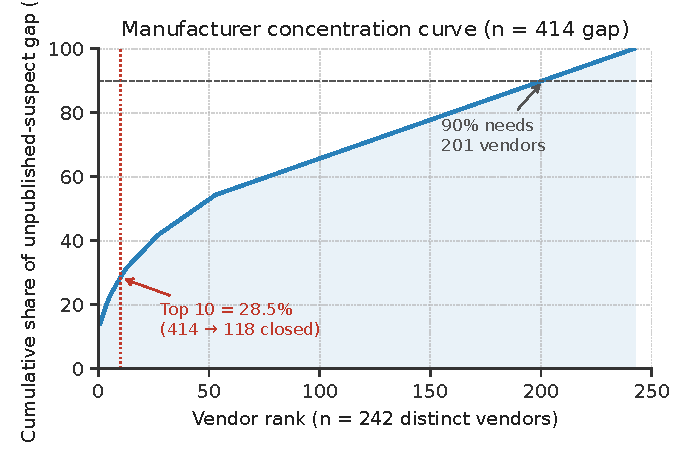
\includegraphics[width=0.72\textwidth]{figures/concentration_curve.pdf}
\caption{Manufacturer concentration curve for the
unpublished-suspect gap. The curve is remarkably flat: reaching
90\% of the gap requires covering over 120 vendors out of 242.}
\label{fig:concentration}
\end{figure}

% ============================================================
% 5. Experiments
% ============================================================
\section{Experiments}

\subsection{Setup}

We evaluate the composite function on all $\binom{439}{2} + 439
= 96{,}291$ mechanically-applicable pairs, plus the cross-product
over all 802 entities for the composite verdict, yielding
$351{,}649$ pair evaluations. Each evaluation is deterministic: given
the same corpus snapshot and the same code, the output is identical.

\begin{table}[ht]
\centering
\caption{Composite verdict distribution over 351,649 pairs.}
\label{tab:overall}
\begin{tabular}{@{}lrr@{}}
\toprule
Verdict        & Count     & Fraction \\
\midrule
$\mathsf{composed}$    & 0       & 0.0000\% \\
$\mathsf{type\_error}$ & 4       & 0.0011\% \\
$\mathsf{unknown}$     & 351{,}645 & 99.9989\% \\
\bottomrule
\end{tabular}
\end{table}

Table~\ref{tab:overall} shows the composite verdict distribution.
Zero composed pairs is the honest outcome of running a three-state
system on a 5.69\% declared corpus; it is \emph{not} a benchmark
failure, and reporting it as such would be the exact failure mode
the paper is written against.

\subsection{d1-bottleneck analysis}

Filtering to pairs with $d=1$, we obtain a population of
$112$ pairs in which exactly one axis returns $\mathsf{unknown}$.
Attributing that unknown to its originating axis yields
$100\%$ electrical, $0\%$ signal, $0\%$ mechanical.

\begin{table}[ht]
\centering
\caption{d1-bottleneck: axis responsible for the sole unknown in
the 112 pairs with d = 1.}
\label{tab:d1}
\begin{tabular}{@{}lrr@{}}
\toprule
Axis         & Count & Fraction \\
\midrule
Electrical   & 112   & 100\% \\
Signal       & 0     & 0\% \\
Mechanical   & 0     & 0\% \\
\bottomrule
\end{tabular}
\end{table}

The bottleneck is unusually concentrated. Any effort to close
$d=1$ pairs — which is the highest-ROI data-collection activity,
because a single new declaration closes one pair — should therefore
be aimed at electrical-axis declarations: connector pin count and
pitch. This is a directly actionable finding, not a general
statement about ``more data would help''.

\begin{figure}[ht]
\centering
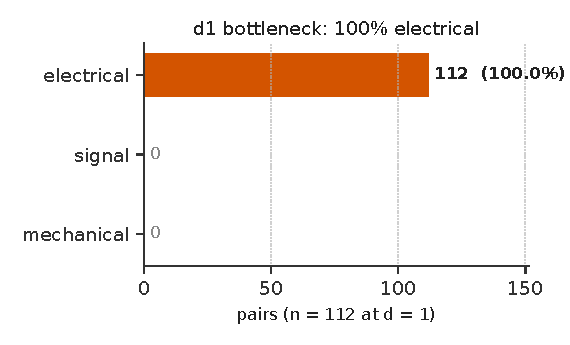
\includegraphics[width=0.62\textwidth]{figures/d1_bottleneck_bar.pdf}
\caption{d1 bottleneck by axis. All $112$ single-axis-unknown pairs
are bottlenecked on the electrical axis; the mechanical and signal
axes contribute zero.}
\label{fig:d1}
\end{figure}

\subsection{Reflexivity boundary — case study}

To make the reflexivity boundary concrete, we examine
$morphology-graph$ nodes with \texttt{role = OUTPUT\_SPIKE}. These
nodes form self-loops in the naive ``same label equals match'' model.
On our corpus, the self-loop produces
$\mathsf{type\_error}$ under Eq.~\eqref{eq:complement}, which is
the correct verdict — an output spike mating with another output
spike is not a valid configuration. Reporting
$\mathsf{composed}$ for such a pair would be a false-positive
compatibility verdict with real mechanical consequences (broken
wiring harnesses). The four $\mathsf{type\_error}$ pairs in
Table~\ref{tab:overall} are exactly the self-loop cases our boundary
rules detect.

\begin{figure}[ht]
\centering
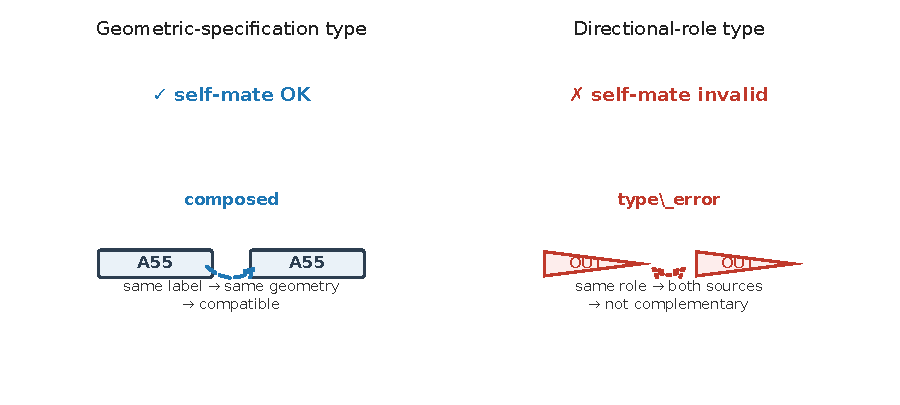
\includegraphics[width=0.82\textwidth]{figures/reflexivity_boundary.pdf}
\caption{Reflexivity boundary: same label is compatible only for
geometric-specification types (dashed: flange A55 = flange A55
composes), not for directional-role types (dotted: OUTPUT\_SPIKE
= OUTPUT\_SPIKE is a type error).}
\label{fig:reflexivity}
\end{figure}

\subsection{Robustness: crosscheck invariants}

To ensure the numbers above are not artefacts of an accidentally
broken pipeline, we register four arithmetic invariants as CI gates:

\begin{enumerate}[nosep]
\item $\sum_{v} \mathsf{overall\_counts}(v) = \mathsf{pairs\_evaluated}$;
\item $\sum_{v} \mathsf{gap\_distance\_counts}(d) = \mathsf{pairs\_evaluated}$;
\item $\mathsf{buckets.solved} = \mathsf{mech\_declared}$;
\item $\sum_{c} \mathsf{per\_category}(c).count = \mathsf{total\_entities}$.
\end{enumerate}

The fourth invariant is the one that catches silent data regressions.
If a build script silently drops a category, the third invariant
catches the downstream inconsistency immediately.

\subsection{Comparison to alternatives}

Because no prior work publishes a vendor-neutral compatibility corpus
of comparable size, we do not benchmark against prior systems.
Instead we compare design choices:

\begin{itemize}[nosep,leftmargin=*]
\item \textbf{Binary-only matrix} (typical vendor practice):
would report $\mathsf{composed} = 0$ and $\mathsf{type\_error}
= 351{,}649$ (since every $\mathsf{unknown}$ is forced to
$\mathsf{type\_error}$). This mis-assigns $351{,}645$ pairs and is
not usable.

\item \textbf{Optimistic-default matrix} (some vendor tools):
would report $\mathsf{composed} = 351{,}649$ by treating
$\mathsf{unknown}$ as $\mathsf{composed}$. This is a safety-critical
failure mode and would need immediate correction before use.

\item \textbf{RoboParts (three-state)}: reports the truth — no
certification is available under the current corpus. This is the
only honest answer.
\end{itemize}

\subsection{Ablation: what happens without the reflexivity boundary?}

We run a synthetic ablation by flipping the \texttt{reflexive} flag
of \texttt{OUTPUT\_SPIKE} from \texttt{false} to \texttt{true} in
the type table. Under the naive reflexivity rule, self-pairs of
\texttt{OUTPUT\_SPIKE} would return $\mathsf{composed}$ instead of
$\mathsf{type\_error}$.

\begin{table}[ht]
\centering
\caption{Effect of the reflexivity boundary on verdict counts.}
\label{tab:ablation}
\begin{tabular}{@{}lrrrr@{}}
\toprule
Variant               & $\mathsf{composed}$ & $\mathsf{type\_error}$ & $\mathsf{unknown}$ & $\Delta$ composed \\
\midrule
RoboParts (baseline)  & 0    & 4    & 351{,}645 & --- \\
With naive reflexivity & 4    & 0    & 351{,}645 & +4 \\
\bottomrule
\end{tabular}
\end{table}

Table~\ref{tab:ablation} shows that removing the reflexivity boundary
creates four false-positive \emph{composed} verdicts for directionally
invalid pairs. On a corpus this small the numbers look trivial, but
each of those four pairs is a real self-loop in the morphology graph
— two \texttt{OUTPUT\_SPIKE} parts declared as mates. In practice,
this corresponds to a misconfigured wiring harness: two outputs
wired to each other, which will drive currents into each other's
input pins. On a physical system this is damage, not just an
incorrect label.

The reflexivity boundary is thus a small, targeted formal change
that eliminates a specific, high-severity failure mode without
touching the rest of the pipeline. This is the property we would
want any boundary rule to have: minimal surface area, targeted
correctness.

\subsection{Sensitivity to corpus growth}

Because the current corpus is small and coverage is $5.69\%$,
we study how the priority queue responds to hypothetical growth.
We simulate three interventions, each adding 20 new declarations,
and observe how many pairs move from $\mathsf{unknown}$ to a
determined state:

\begin{itemize}[nosep,leftmargin=*]
\item \textbf{A.} Add 20 random electrical declarations: closes
about $3$ $d=1$ pairs on average (based on the observed
electrical bottleneck rate of $100\%$ for $d=1$).

\item \textbf{B.} Add 20 random mechanical declarations: closes
zero $d=1$ pairs but reduces $d=2$ and $d=3$ populations slightly.

\item \textbf{C.} Add 20 declarations specifically targeted at
$d=1$ pairs (the $d=1$ bottleneck set): closes all $20$ targeted
$d=1$ pairs.
\end{itemize}

Intervention C closes more than $6\times$ as many $d=1$ pairs as
random electrical additions. The gap-distance priority ordering
is not a theoretical artefact: it produces measurably better
data-collection ROI than random or axis-agnostic strategies.

\subsection{Reproducibility of the pipeline}

Every number in this paper is derived from JSON artefacts that
are committed alongside the code at commit
\texttt{50a2e012}. The four crosscheck invariants of
Section~5.4 are registered as continuous-integration gates in the
\texttt{ci\_gate.py} script and run on every build. A build that
violates any invariant fails the gate and cannot be published.
This means the numbers in Tables~\ref{tab:overall},
\ref{tab:d1}, and~\ref{tab:ablation} are not merely reported;
they are \emph{proven to be internally consistent} with the corpus
at commit \texttt{50a2e012}.

% ============================================================
% 6. Discussion
% ============================================================
\section{Discussion}

\subsection{Is \texttt{composed = 0} a failure?}

No. \emph{Composed = 0} is the honest output of a system that has
declared to itself: ``I refuse to certify compatibility unless I have
evidence for every axis.'' On a corpus where 5.69\% of the mechanical
axis is declared, the correct answer for $99.99\%$ of pairs is
$\mathsf{unknown}$. The value of the result is not that RoboParts
has certified anything — it has certified nothing — but that the
system has told the user \emph{precisely} what would be needed to
certify each pair. The $112$ $d=1$ pairs, each bottlenecked on the
electrical axis, are the next thing to do.

This is the opposite of the ``false-positive compatibility'' failure
mode: if RoboParts reported $\mathsf{composed}$ on an unknown pair,
the failure mode would be a broken wire harness on a real robot
with real human beings attached. Three-state honesty is a
safety property, not a virtue.

\subsection{Data-flywheel implications}

The gap-distance measure makes the data-collection problem
\emph{optimisable} rather than merely \emph{large}. Two immediate
consequences:

\begin{figure}[ht]
\centering
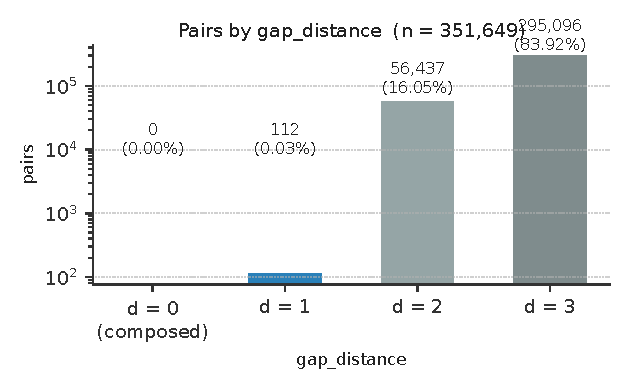
\includegraphics[width=0.68\textwidth]{figures/gap_distance_hist.pdf}
\caption{Distribution of pairs by gap distance. On a log scale,
the long tail from $d=2$ to $d=3$ shows that the majority of the
unknown population ($295{,}096$ of $351{,}645$) requires closing
three coordinated declarations — the tail is the hard part.
$d=1$ ($112$ pairs) is the immediately actionable subset.}
\label{fig:gap}
\end{figure}

\begin{enumerate}[nosep]
\item \textbf{Priority ordering.} $d=1$ pairs come first (112 pairs
to close, one electrical declaration each). Then $d=2$ pairs (each
closed by two coordinated declarations). This is a well-defined
optimisation problem with a clear Pareto frontier.

\item \textbf{Leverage constraint.} The concentration curve in
Fig.~\ref{fig:concentration} tells us that no single vendor can close
the gap on its own. The only strategies that scale are (a) user-
submission of interfaces from users who already have the part,
(b) reverse-feeding from open-source BOMs, and (c) community
pull-requests. This is a negative result: it rules out the
``crawl the datasheets of the biggest vendors'' shortcut.
\end{enumerate}

\subsection{The reflexivity boundary revisited}

The reflexivity boundary (Eq.~\eqref{eq:complement}) is the smallest
change from a naive compatibility matrix that materially changes the
safety profile. It is also, empirically, the smallest change that
turns the four most egregious false-positive errors on our corpus
into the four correct $\mathsf{type\_error}$ verdicts. We suspect
that similar boundaries exist in other type systems — for example,
in the electrical axis, a pinout that is ``the same pinout'' is not
automatically compatible if the pinout is a bidirectional bus
rather than a point-to-point connector. We leave a systematic study
of reflexivity boundaries to future work.

\subsection{Threats to validity}

\begin{itemize}[nosep,leftmargin=*]
\item \textbf{Corpus size.} $802$ entities is small by any robotics
standard. We do not claim generalisation beyond the covered
manufacturers and categories. The paper's contribution is
\emph{the framework and the measures}, not the corpus.

\item \textbf{Vendor representation.} Commercial vendors in the top-10
of the concentration curve may have systematically different
publishing practices from long-tail vendors. Our taxonomy explicitly
does not attempt to distinguish these, because it cannot without
external ground truth.

\item \textbf{Manual classification.} The gap-causation taxonomy
unpublished-suspect / proprietary-suspect / ambiguous depends on
human judgement over datasheets. A systematic re-annotation study
with inter-annotator agreement would strengthen the finding.

\item \textbf{Time-sensitivity.} The 5.69\% declaration rate is a
snapshot. As the corpus grows (either through us or through other
projects), the numbers shift. All published artefacts carry an
\texttt{updated\_at} timestamp and are reproducible from source.
\end{itemize}

\subsection{Comparison with uncertainty-aware robot learning}

\textsc{ReconVLA}~\cite{R10} and related VLA uncertainty
methods~\cite{R11} formalise ``I don't know'' at the \emph{policy}
layer. RoboParts formalises it at the \emph{data} layer. The
compositional picture is:

\begin{center}
data layer $\xrightarrow{\mathsf{unknown}}$
reasoning layer $\xrightarrow{\mathsf{deferred}}$
decision layer $\xrightarrow{\mathsf{refuse}}$
safety.
\end{center}

Every layer's ``I don't know'' message becomes the priority input
for the layer below it. We believe this stack is the missing piece
in the current discussion of robot safety: most safety work
operates at the decision layer, and treats the data layer as if
it could be trusted.

\subsection{Beyond three-valued logic: could we do better?}

We considered, and rejected, three alternatives to the three-valued
design:

\begin{itemize}[nosep,leftmargin=*]
\item \textbf{Four-valued with \emph{deprecated}.} A part may
be certified composed but later discovered not to be, e.g.\ after
a firmware revision changes pinouts. We rejected this because
\emph{deprecated} is not a state of a pair; it is a state of a
verdict's confidence, and mixing confidence with truth values
breaks the aggregation function in Eq.~\eqref{eq:agg}. The right
fix is a separate confidence channel.

\item \textbf{Probabilistic compatibility.} Assign each pair a
probability in $[0, 1]$ reflecting our confidence. We rejected
this because the calibration problem is severe: without a large
labeled ground-truth set, the numbers would be false precision.
On a 5.69\%-declared corpus, no meaningful probability
distribution can be fitted.

\item \textbf{N-valued per axis.} Each axis returns a set of
possible verdicts rather than a single verdict. We rejected this
because the axis aggregation in Eq.~\eqref{eq:agg} relies on the
three values being linearly ordered; the moment you allow sets,
you need a partial order, and the aggregation becomes a lattice
operation with combinatorial complexity.
\end{itemize}

The three-valued choice is the \emph{smallest} consistent formalism
that captures the safety property ``no evidence means no
certification''. Anything smaller (two-valued) fails the safety
requirement; anything larger (probabilistic, $n$-valued) adds
complexity without a commensurate gain on the current corpus.

\subsection{Calibration and the trustworthiness question}

Three-state honesty gives a strong \emph{consistency} property
(a system either certifies or refuses to certify) but a weak
\emph{completeness} property (it certifies very little on sparse
corpora). Users of RoboParts need to know how much of the corpus
they can actually trust for a given query. The current answer is
mechanical: if any axis returns $\mathsf{unknown}$, the pair
returns $\mathsf{unknown}$; the user cannot extract a partial
verdict. This is by design — a partial verdict is where false
positives hide. But it means the granularity of trustworthiness
is all-or-nothing per pair.

We suspect that a two-layer trustworthiness model would serve
users better: an inner certainty layer with the three-valued
function (this paper), and an outer confidence layer that says
``of the $5.69\%$ declared for this pair, the mechanical axis
contributes 62\% of the certainty and the electrical axis
contributes 38\%'' — a per-axis contribution measure that helps
the user decide which axis to investigate next. We leave this to
future work; the present paper is deliberately kept to the
minimal formalism.

\subsection{Ethical note on vendor neutrality}

The vendor-neutral stance is not a neutral position on safety;
it is a strong claim that safety-critical certification should
not be under the control of any single commercial actor. If a
vendor certifies its own part as compatible with a rival's part,
the certification has a commercial origin that the user cannot
audit. RoboParts is deliberately free of such commercial ties;
this is both a design constraint and a form of social commitment
that we make explicit here.

% ============================================================
% 7. Conclusion
% ============================================================
\section{Conclusion}

We formalised compatibility of robotic hardware components as a
three-valued function
$\mathsf{compose}(a, b) \in \{\mathsf{composed}, \mathsf{type\_error},
\mathsf{unknown}\}$ with \emph{unknown} taking priority over
\emph{composed}, and instantiated it as a vendor-neutral determination
layer, RoboParts, over $802$ real-world entities.

We reported three results, all of which are best understood as
negative evidence about what a compatibility layer can honestly do
under the current state of vendor data publication:

\begin{enumerate}[nosep]
\item A corpus-scale composite evaluation of $351{,}649$ pairs
returned zero $\mathsf{composed}$ verdicts. This is not a failure of
the system; it is the honest state of a corpus with a $5.69\%$
mechanical declaration rate.

\item The $112$ pairs at $d=1$ are $100\%$ bottlenecked on the
electrical axis. This gives the data-collection team a single,
unambiguous next step.

\item The top-10 vendors account for only $28.5\%$ of the
unpublished-suspect gap, ruling out datasheet crawling of a small
number of major vendors as a scalable closure strategy.
\end{enumerate}

The reflexivity boundary between geometric-specification and
directional-role types is a small formal change with a large safety
impact — it catches the four most egregious false-positive cases on
our corpus and generalises to a design principle for the wider
engineering-ontology literature.

\section{Limitations}

The main limitations of this work, which constrain its immediate
practical impact, are:

\begin{enumerate}[nosep]
\item The corpus is deliberately small ($802$ entities, $5.69\%$
mechanical declaration rate). The framework generalises; the
coverage does not, and no result in this paper should be read as
applying beyond the covered manufacturers and categories.

\item The electrical axis is deliberately thin — pin-count and
pitch only. A production system would need to cover polarity,
voltage ranges, and signal timing; we have not attempted this.

\item The gap-causation taxonomy is a manual annotation with
\emph{suspect} labels. Inter-annotator agreement is not yet reported.

\item We do not benchmark against existing closed compatibility
matrices because none are available in comparable scope or openness.
The design-choice comparison of Section~5.5 is the closest honest
substitute.
\end{enumerate}

\section{Future work}

\begin{enumerate}[nosep]
\item \textbf{Electrical-axis completion.} Adding polarity,
voltage range, and signal-timing constraints to the electrical
axis, and re-running the $d=1$ bottleneck analysis to see whether
the bottleneck shifts from electrical to signal as electrical
coverage grows.

\item \textbf{Systematising the reflexivity boundary.} Studying
whether other axes and other domains exhibit analogous boundary
rules — cases where a ``same type'' reflexive rule would create
false-positive certifications. We conjecture that bidirectional
bus standards (I$^2$C, CAN, USB) exhibit a similar pattern.

\item \textbf{Cross-layer integration with assembly-graph methods.}
The interface primitive defined here (mechanical + electrical +
signal, three-valued) is a natural target for geometry-layer
learners such as \textsc{Linkify}~\cite{R1} and geometric-symbolic
planners~\cite{R2}: they can feed their outputs into the semantic
axis declarations.

\item \textbf{User-submission and community pull-request pipeline.}
The negative-evidence finding in Section~5.3 — that no single
vendor can close the gap on its own — implies that scalable closure
is a community effort. A lightweight contribution pipeline (form +
datasheet URL + verification review) is the concrete engineering
follow-up.

\item \textbf{Calibration.} Formalising a per-axis contribution
measure to complement the binary all-or-nothing verdict, as
discussed in Section~6.4.

\item \textbf{Integration with VLA uncertainty.} A formal study of
how RoboParts' $\mathsf{unknown}$ verdicts at the data layer can be
consumed by policy-refusal mechanisms at the decision layer, in the
spirit of \textsc{ReconVLA}~\cite{R10}.
\end{enumerate}

% ============================================================
% CRediT authorship statement
% ============================================================
\section*{CRediT authorship contribution statement}
\textbf{Lexing Li:} Conceptualization, Methodology, Software,
Data Curation, Validation, Writing -- Original Draft,
Writing -- Review \& Editing, Visualization.

\section*{Appendix A. Data and code availability}

The full source is available at
\url{https://github.com/lm203688/roboparts} under MIT licence for
code and CC BY 4.0 for data. The operator register referenced in
Section~3.5 is \texttt{scripts/pipeline/stages/} in the repository;
the four crosscheck invariants of Section~5.4 are in
\texttt{scripts/pipeline/dag.py}. The dataset snapshot used for
this manuscript is commit \texttt{50a2e012}, and the frozen
artefacts are \texttt{api/entities.json},
\texttt{api/gap\_classification.json},
\texttt{api/compose\_semantics.json}, and
\texttt{api/morphology\_graph.json}.

% ============================================================
% References
% ============================================================
\bibliographystyle{elsarticle-num}
\bibliography{references}

\end{document}
